\documentclass{standalone}
\usepackage{tikz}
\usetikzlibrary{automata,positioning}
\begin{document}
\begin{tikzpicture}[->,>=stealth,auto,node distance=2.5cm,semithick,every state/.style={minimum width=1cm, minimum height=1cm, text width=0.75cm,align=center}]
\node[state, initial] (12) at (0,5.0) {12};
\node[state] (1) at (10,5.0) {1};
\node[state] (2) at (20,5.0) {2};
\node[state] (3) at (30,5.0) {3};
\node[state] (4) at (50,5.0) {4};
\node[state] (5) at (60,5.0) {5};
\node[state] (6) at (70,5.0) {6};
\node[state] (7) at (80,5.0) {7};
\node[state] (8) at (80,10.0) {8};
\node[state] (9) at (90,5.0) {9};
\node[state, accepting] (10) at (90,10.0) {10};
\node[state] (11) at (40,5.0) {11};
\path (12) edge node[midway, sloped, above] {54} (1);
\path (1) edge node[midway, sloped, above] {T54} (2);
\path (2) edge node[midway, sloped, above] {T54} (3);
\path (3) edge node[midway, sloped, above] {T232} (11);
\path (11) edge node[midway, sloped, above] {101} (4);
\path (4) edge node[midway, sloped, above] {Tran} (5);
\path (5) edge node[midway, sloped, above] {Tra} (6);
\path (6) edge node[midway, sloped, above] {Tra} (7);
\path (6) edge node[midway, sloped, above] {Tr} (8);
\path (8) edge node[midway, sloped, above] {Tra} (9);
\path (8) edge node[midway, sloped, above] {Tra} (10);
\end{tikzpicture}
\end{document}